\documentclass[14pt]{article}

\usepackage[utf8]{inputenc}
\usepackage[T1]{fontenc}
\usepackage{lmodern}
\usepackage[english]{babel}
\usepackage{cite}
\usepackage{amssymb}
\usepackage{amsfonts}
\usepackage{amsmath}
\usepackage{mathrsfs}
\usepackage{enumerate}
\usepackage{fullpage}
\usepackage{times}
\usepackage{balance}
\usepackage{graphicx}

\usepackage[skip=14pt,font=Large]{caption}
\captionsetup[figure]{labelformat=empty}
\usepackage{subcaption}


\usepackage{hyperref}
\usepackage{dsfont}
\usepackage{fullpage}
\usepackage{float}
\usepackage{color}

\usepackage{titlesec}

\usepackage{footmisc}% http://ctan.org/pkg/footmisc
\usepackage{relsize}% http://ctan.org/pkg/relsize
\renewcommand\footnotelayout{\small}


\titleformat*{\section}{\LARGE\bfseries}
\titleformat*{\subsection}{\Large\bfseries}
\titleformat*{\subsubsection}{\large\bfseries}
\titleformat*{\paragraph}{\large\bfseries}
\titleformat*{\subparagraph}{\large\bfseries}

\usepackage{enumitem}
\setlist[itemize]{label=}

\hypersetup{
    colorlinks,%
    citecolor=black,%
    filecolor=black,%
    linkcolor=black,%
    urlcolor=black
}

\begin{document}
\fontsize{14}{14}\selectfont
\noindent
img/example.png\\[.5cm]
Agenda
\begin{enumerate}
\item Opening
\item Approval of agenda
\item Review of previous minutes
\item Actions taken since previous meeting
\end{enumerate}
\noindent
img/lists/1.png
\begin{itemize}
\setlength{\itemsep}{0pt}
\setlength{\parskip}{0pt}
\setlength{\parsep}{0pt}
\item $\bullet\ $ Pick up Peter
\item $\bullet\ $ Go to the supermarket, buy:
\begin{itemize}
\setlength{\itemsep}{0pt}
\setlength{\parskip}{0pt}
\setlength{\parsep}{0pt}
\item $\bullet\ $ Eggs
\item $\bullet\ $ Milk
\item $\bullet\ $ Coffee
\begin{itemize}
\setlength{\itemsep}{0pt}
\setlength{\parskip}{0pt}
\setlength{\parsep}{0pt}
\item $\bullet\ $ Ground coffee
\item $\bullet\ $ Whole beans
\end{itemize}
\end{itemize}
\item $\bullet\ $ Call mother
\end{itemize}
\noindent
img/lists/1\_2.png
\begin{itemize}
\setlength{\itemsep}{1pt}
\setlength{\parskip}{0pt}
\setlength{\parsep}{0pt}
\item $\bullet\ $ Pick up Peter
\item $\bullet\ $ Go to the supermarket, buy:
\item $\bullet\bullet\ $ Eggs
\item $\bullet\bullet\ $ Milk
\item $\bullet\bullet\ $ Coffee
\item $\bullet\bullet$$\bullet\ $ Ground coffee
\item $\bullet\bullet$$\bullet\ $ Whole beans
\item $\bullet\ $ Call mother
\end{itemize}
\noindent

\begin{verbatim}
img/lists/3_1.png

* Pick up Peter
** Go to the supermarket, buy:
** Eggs
** Milk
** Coffee
*** Ground coffee
*** Whole beans
* Call Mother













img/lists/3_2.png
  
* Pick up Peter
* Go to the supermarket, buy:
  * Eggs
  * Milk
  * Coffee
    * Ground coffee
    * Whole beans
* Call Mother

\end{verbatim}
\noindent
img/styling/bold/1.png\\[.5cm]
I am \textbf{sure} about \textbf{that}\\[.5cm]
img/styling/bold/2\_2.png\\[.5cm]
I am \textit{sure} about \textit{that}\\[.5cm]
img/styling/bold/2\_3.png\\[.5cm]
I am \underline{sure} about \underline{that}\\[.5cm]
img/styling/italic/1.png\\[.5cm]
I did read the entire \textit{Harry Potter} series\\[.5cm]
img/styling/italic/2\_2.png\\[.5cm]
I did read the entire \textbf{Harry Potter} series\\[.5cm]
img/styling/italic/2\_3.png\\[.5cm]
I did read the entire \underline{Harry Potter} series\\[.5cm]



\begin{verbatim}
img/styling/bold/3_1.png

I am *sure* about *that*


img/styling/bold/3_2.png

I am **sure** about **that**


img/styling/bold/3_3.png

I am __sure__ about __that__





img/styling/italic/3_1.png

I did read the entire //Harry Potter// series


img/styling/italic/3_2.png

I did read the entire _Harry Potter_ series


img/styling/italic/3_3.png

I did read the entire *Harry Potter* series

\end{verbatim}
\noindent
img/styling/color/1.png\\[.5cm]
All \textcolor{red}{nouns} are marked with red in this \textcolor{red}{sentence}

\begin{verbatim}

img/styling/color/3_1.png

All %red nouns% are marked with red in this %red sentence%


img/styling/color/3_2.png

All <red nouns> are marked with red in this <red sentence>


img/styling/color/3_3.png

All #red nouns# are marked with red in this #red sentence#


img/styling/color/2.png

Switching text and colors: %red green% and %blue yellow%


\end{verbatim}
\noindent
img/styling/color/2\_1.png\\[.5cm]
Switching text and colors: \textcolor{red}{green} and \textcolor{blue}{yellow}\\[.5cm]
img/styling/color/2\_2.png\\[.5cm]
Switching text and colors: \textcolor{green}{red} and \textcolor{yellow}{blue}\\[1.5cm]
img/sections/1.png
\section*{English language}
English is a West Germanic language.
\subsection*{Vocabulary}
English vocabulary has changed considerably over the centuries.
\subsubsection*{Number of words in English}
The vocabulary of English is undoubtedly very large.
\subsection*{History}
English originated in the dialects of North Sea Germanic.

\newpage
\begin{verbatim}
img/sections/3_1.png

====== English language
English is a West Germanic language.

===== Vocabulary
English vocabulary has changed considerably over the centuries.

==== Number of words in English
The vocabulary of English is undoubtedly very large.

===== History
English originated in the dialects of North Sea Germanic.



img/sections/3_2.png

================
English language
================
English is a West Germanic language.

----------
Vocabulary
----------
English vocabulary has changed considerably over the centuries.

Number of words in English
==========================
The vocabulary of English is undoubtedly very large.

-------
History
-------
English originated in the dialects of North Sea Germanic.

\end{verbatim}
\newpage
\begin{verbatim}
img/sections/3_3.png

== English language
English is a West Germanic language.

=== Vocabulary
English vocabulary has changed considerably over the centuries.

==== Number of words in English
The vocabulary of English is undoubtedly very large.

=== History
English originated in the dialects of North Sea Germanic.



img/sections/3_4.png

English language
================
English is a West Germanic language.

Vocabulary
----------
English vocabulary has changed considerably over the centuries.

Number of words in English
..........................
The vocabulary of English is undoubtedly very large.

History
-------
English originated in the dialects of North Sea Germanic.


\end{verbatim}
\noindent
img/references/1.png\\[.5cm]
The first Harry Potter book$^1$ was written in 1997.\\[1cm]
$^1$ by J.K. Rowling

\newpage
\begin{verbatim}
img/references/3_1.png

The first Harry Potter book[#]_ was written in 1997.

[#]: by J.K. Rowling


img/references/3_2.png

The first Harry Potter book%footnote by J.K. Rowling% was
written in 1997.


img/references/3_3.png

The first Harry Potter book^[#] was written in 1997.

[#]: by J.K. Rowling

\end{verbatim}
\noindent
img/references/2\_2.png\\[.5cm]
The first Harry Potter book[1] was written in 1997.\\[1cm]
[1]: by J.K. Rowling\\[1cm]
img/references/2\_3.png\\[.5cm]
The first Harry Potter book$_1$ was written in 1997.\\[1cm]
$_1$ by J.K. Rowling
\newpage
img/figures/1.png\\[.5cm]
\begin{figure}[H]
\begin{center}
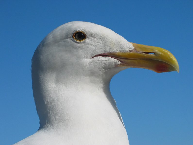
\includegraphics[scale=1]{../../img/gull.png}
\caption{A picture of a gull.}
\end{center}
\end{figure}
\noindent
\begin{verbatim}
img/figures/3_1.png

![my_image]

[my_image]: gull.jpg "A picture of a gull."


img/figures/3_2.png

!(gull.jpg "A picture of a gull.")


img/figures/3_3.png

!gull.jpg(A picture of a gull.)!

\end{verbatim}
\newpage
\noindent
img/figures/2\_2.png\\[.5cm]
A picture of a gull.
\begin{figure}[H]
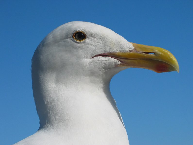
\includegraphics[scale=1]{../../img/gull.png}
\end{figure}
\newpage
\noindent
img/figures/2\_3.png\\[.5cm]
\begin{figure}[H]
\begin{center}
\fontsize{14}{14}\selectfont
A picture of a gull.\\
\setlength{\itemsep}{12pt}
\setlength{\parskip}{12pt}
\setlength{\parsep}{12pt}

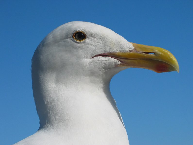
\includegraphics[scale=1]{../../img/gull.png}
\end{center}
\end{figure}
\noindent
img/symbols/1.png\\[.5cm]
$\beta\ \ \  \alpha$
\begin{verbatim}

img/symbols/3_1.png

#beta  #alpha


img/symbols/3_2.png

#B  #a


img/symbols/3_3.png

#B# #a#


img/symbols/3_4.png

#beta# #alpha#

\end{verbatim}
\noindent
img/symbols/2\_2.png\\[.5cm]
\textbf{B} \ \textbf{a}\\[.5cm]
img/symbols/2\_3.png\\[.5cm]
\textit{B} \ \textit{a}\\[.5cm]
img/symbols/2\_4.png\\[.5cm]
\textbf{\#B} \ \textbf{\#a}\\[1cm]
img/tables/1.png (600dpi)
\begin{table}[H]
\begin{tabular}{| l | l |}
\hline
Year & President \\
\hline
1789 & George Washington \\
\hline
1797 & John Adams \\
\hline
1801 & Thomas Jefferson \\
\hline
\end{tabular}
\end{table}
\noindent
\begin{verbatim}
img/tables/3_1.png

| Year  | President          |
| ----- | ------------------ |
| 1789  | George Washington  |
| 1797  | John Adams         |
| 1801  | Thomas Jefferson   |


img/tables/3_2.png

+----------------------------+
| Year  | President          |
+============================+
| 1789  | George Washington  |
+----------------------------+
| 1797  | John Adams         |
+----------------------------+
| 1801  | Thomas Jefferson   |
+----------------------------+


img/tables/3_3.png

^ Year  ^ President          ^
| 1789  | George Washington  |
| 1797  | John Adams         |
| 1801  | Thomas Jefferson   |

\end{verbatim}


img/math/1.png \\[.5cm]
$x = \frac{\sqrt{b^2-4ac}}{\lfloor2a\rfloor}$

\begin{verbatim}


img/math/3_1.png

x = {sqrt{b sup 2 - 4ac}} over floor{2a}



img/math/3_2.png

x = \frac{\sqrt{b^2 - 4ac}}{\lfloor 2a \rfloor}



img/math/3_3.png

x = (sqrt(b^2 - 4ac))/floor(2a)
\end{verbatim}

\end{document}
